
\section{mcliqueInfo.rb 列挙されたクリークの各種情報\label{sect:mcliqueInfo}}

mclique.rbコマンドで列挙されたクリークについての各種情報を出力する。
本コマンドの主な目的は、クリーク同士の接続関係についての各種情報を出力することにある。

mclique2g.rbコマンドの解説で用いたグラフを図\ref{fig:mcinfo_1}に再掲する。
このグラフから得られる極大クリークは4つ存在する。
これら4つのクリークそれぞれについて、表\ref{tbl:mcinfo_1}に示す5つの情報を出力する。

\begin{table}[htbp]
\begin{center}
\caption{本コマンドの出力結果\label{tbl:mcinfo_1}}
%{\small
\begin{tabular}{lll}
\hline
出力項目名&内容&id=1(\{$d,e,f$\}の例) \\
\hline
nSize      & 節点数                    & 3 (節点$d,e,f$の3つ)\\
eSize      & 枝数(nSize$*$(nSize-1)/2) & 3 $(3*2/2=3)$\\
extNodes   & 外部接続節点数            & 5 (図\ref{fig:mcinfo_3}右) \\
extEdges   & 外部接続枝数              & 7 (図\ref{fig:mcinfo_3}左) \\
extCliques & 外部接続クリーク数        & 3 (図\ref{fig:mcinfo_2}) \\
\hline
\end{tabular} 
\end{center}
\end{table}


\begin{figure}[htbp]
\begin{center}
\begin{tabular}{cc}

\begin{minipage}{0.5\hsize}
\begin{center}
\includegraphics[scale=0.3]{./mcinfo_1.eps}
\caption{極大クリーク列挙の対象となるグラフ。
4つの極大クリーク\{a,b,c,d\}(id=0)、\{d,e,f\}(id=1)、\{e,f,g\}(id=2)、\{e,f,h\}(id=3)を含んでいる。\label{fig:mcinfo_1}}
\end{center}
\end{minipage}

\begin{minipage}{0.5\hsize}
\begin{center}
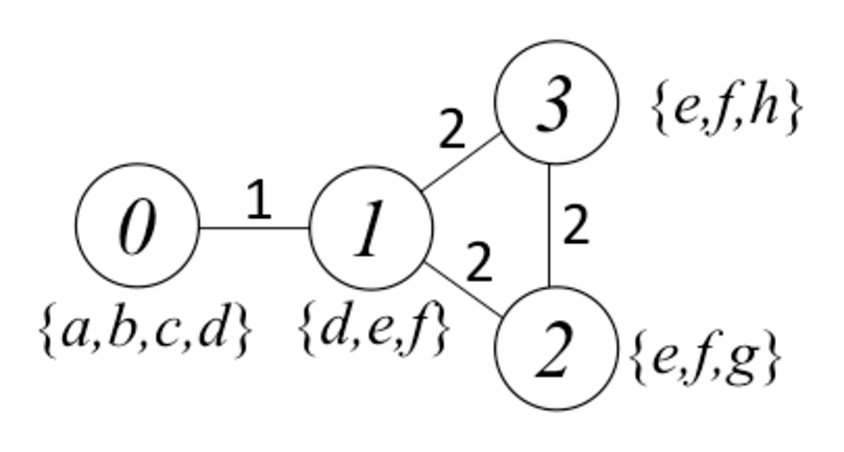
\includegraphics[scale=0.3]{./mcinfo_2.eps}
\caption{極大クリークグラフ。図\ref{fig:mcinfo_1}のクリークidを節点としたグラフ。
枝は共通の節点数を表している。
id=1のクリークは3つのクリークに直接の接続があることがわかる。
なお、このグラフを出力したければ\ref{sect:mclique2g}節を参照のこと。
\label{fig:mcinfo_2}}
\end{center}
\end{minipage}

\end{tabular} 
\end{center}
\end{figure} 

\begin{figure}[htbp]
\begin{center}
\begin{tabular}{c}

\begin{minipage}{0.5\hsize}
\begin{center}
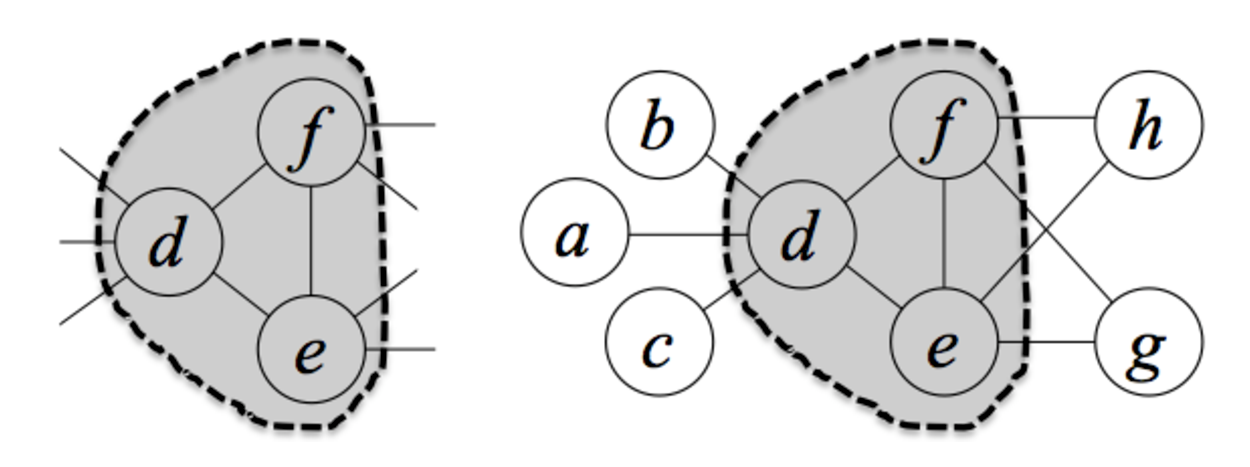
\includegraphics[scale=0.3]{./mcinfo_3.eps}
\caption{クリークid=1(グレーで示された領域)から外の節点へと接続される枝は7本ある(左図)。
クリークid=1(グレーで示された領域)から接続される節点数は5である(右図)。
\label{fig:mcinfo_3}}
\end{center}
\end{minipage}

\end{tabular} 
\end{center}
\end{figure} 

本コマンドの入力データは、\ref{sect:mclique2g}節に示したmclique2g.rbコマンド
と同様で、表\ref{tbl:clique2g_1}に示されるような、
クリークIDと節点の2項目から構成されるCSV形式データである。
そして、出力結果は、表\ref{tbl:mcinfo_3}に示されるように、
極大クリーク毎に表\ref{tbl:mcinfo_1}に示される情報が出力される。

\begin{table}[htbp]
\begin{center}
\begin{tabular}{cc}

\begin{minipage}{0.3\hsize}
\begin{center}
\caption{入力データ\label{tbl:mcinfo_2}}
{\small
\begin{tabular}{cc}
\hline
id&node \\
\hline
0&a \\
0&b \\
0&c \\
0&d \\
1&d \\
1&e \\
1&f \\
2&e \\
2&f \\
2&g \\
3&e \\
3&f \\
3&h \\
\hline
\end{tabular} 
}
\end{center}
\end{minipage}

\begin{minipage}{0.7\hsize}
\begin{center}
\caption{出力結果\label{tbl:mcinfo_3}}
{\small
\begin{tabular}{cccccc}
\hline
id&nSize&eSize&extNodes&extEdges&extCliques \\
\hline
0&4&6&2&2&1 \\
1&3&3&5&7&3 \\
2&3&3&2&4&2 \\
3&3&3&2&4&2 \\
\hline
\end{tabular} 
}
\end{center}
\end{minipage}

\end{tabular} 
\end{center}
\end{table} 



%これらのクリークと図に示された元のグラフとの関係について本コマンドは表\ref{tbl:ci_result}に示されるような結果を出力する。
%idはクリークを識別するIDで(図\ref{fig:ci_graph}のキャプションに記載)、それぞれのクリークについて表\ref{tbl:ci_flds}に示される情報を出力する。


\subsection{書式}
\begin{verbatim}
書式) mcliqueInfo.rb i= [id=] [f=] [m=] [F=] o= [T=] [--help]
  i=     : クリークデータファイル名
  id=    : クリークID項目名(デフォルト:"id")
  f=     : クリークを構成する節点項目名(デフォルト:"node")

  T= : ワークディレクトリ(default:/tmp)
  --help : ヘルプの表示
\end{verbatim}

\subsection{利用例}
\subsubsection*{例1: Basic Example}

Example illustrated in the previous section.


\begin{Verbatim}[baselinestretch=0.7,frame=single]
$ more clique.csv
id,node
0,a
0,b
0,c
0,d
1,d
1,e
1,f
2,e
2,f
2,g
3,e
3,f
3,h
$ mcliqueInfo.rb i=clique.csv o=result1.csv id=id f=node
#END# /Users/stephane/.rvm/gems/ruby-2.0.0-p247/bin/mcliqueInfo.rb i=clique.csv o=result1.
csv id=id f=node
$ more result1.csv
id,nSize,eSize,extNodes,extEdges,extCliques
0,4,6,2,2,1
1,3,3,5,7,3
2,3,3,2,4,2
3,3,3,2,4,2
\end{Verbatim}


